%% Based on a TeXnicCenter-Template, which was
%% created by Christoph B�rensen
%% and slightly modified by Tino Weinkauf.
%%%%%%%%%%%%%%%%%%%%%%%%%%%%%%%%%%%%%%%%%%%%%%%%%%%%%%%%%%%%%

\documentclass[a4paper,12pt]{scrartcl} %This is a special class provided by the KOMA script, which does a lot of adjustments to adapt the standard LaTeX classes to european habits, change to [a4paper,12pt,twoside] for doublesided layout


%########################### Preferences #################################


% ********* Font definiton ************
\usepackage{t1enc} % as usual
\usepackage[latin1]{inputenc} % as usual
\usepackage{times}		
%\usepackage{mathptmx}  	%mathematical fonts for use with times, I encountered some problems using this package togather with pdftex, which I was not able to resolve

% ********* Graphics definition *******
\usepackage[pdftex]{graphicx} % required to import graphic files
\usepackage{color} %allows to mark some entries in the tables with color
\usepackage{eso-pic} % these two are required to add the little picture on top of every page
\usepackage{everyshi} % these two are required to add the little picture on top of every page

% ********* Defining citation styles *********
\usepackage[backend=bibtex8,style=numeric]{biblatex}
% Select the bibliography file
\addbibresource{sources.bib}

\renewcommand{\floatpagefraction}{0.7} %default:0.5 allows two big pictures on one page

%********** Enybeling Hyperlinks *******
\usepackage[pdfborder=000,pdftex=true]{hyperref}% this enables jumping from a reference and table of content in the pdf file to its target

% ********* Table layout **************
\usepackage{booktabs}	  	%design of table, has an excellent documentation
%\usepackage{lscape}			%use this if you want to rotate the table together with the lines around the table

% ********* Caption Layout ************
\usepackage{ccaption} % allows special formating of the captions
\captionnamefont{\bf\footnotesize\sffamily} % defines the font of the caption name (e.g. Figure: or Table:)
\captiontitlefont{\footnotesize\sffamily} % defines the font of the caption text (same as above, but not bold)
\setlength{\abovecaptionskip}{0mm} %lowers the distace of captions to the figure


% ********* Header and Footer **********
% This is something to play with forever. I use here the advanced settings of the KOMA script

\usepackage{scrpage2} %header and footer using the options for the KOMA script
\renewcommand{\headfont}{\footnotesize\sffamily} % font for the header
\renewcommand{\pnumfont}{\footnotesize\sffamily} % font for the pagenumbers

%the following lines define the pagestyle for the main document
\defpagestyle{cb}{%
(\textwidth,0pt)% sets the border line above the header
{\pagemark\hfill\headmark\hfill}% doublesided, left page
{\hfill\headmark\hfill\pagemark}% doublesided, right page
{\hfill\headmark\hfill\pagemark}%  onesided
(\textwidth,1pt)}% sets the border line below the header
%
{(\textwidth,1pt)% sets the border line above the footer
{{\it Technical University of Vienna}\hfill Andreas Egger}% doublesided, left page
{Andreas Egger\hfill{\it Technical University of Vienna}}% doublesided, right page
{Andreas Egger\hfill{\it Technical University of Vienna}} % one sided printing
(\textwidth,0pt)% sets the border line below the footer
}

%this defines the page style for the first pages: all empty
\renewpagestyle{plain}%
	{(\textwidth,0pt)%
		{\hfill}{\hfill}{\hfill}%
	(\textwidth,0pt)}%
	{(\textwidth,0pt)%	
		{\hfill}{\hfill}{\hfill}%
	(\textwidth,0pt)}

%********** Footnotes **********
\renewcommand{\footnoterule}{\rule{5cm}{0.2mm} \vspace{0.3cm}} %increases the distance of footnotes from the text
\deffootnote[1em]{1em}{1em}{\textsuperscript{\normalfont\thefootnotemark}} %some moe formattion on footnotes

%################ End Preferences, Begin Document #####################

\pagestyle{plain} % no headers or footers on the first page

\begin{document}

\begin{center}

% There might be better solutions for the title page, giving all distances and sizes manually was simply the easiest solution

{\Huge\bf\sf Thesis Notes }

\vspace{4.5cm}

{\Huge\bf\sf Cost aware resource management in }

\vspace{0.5cm}

{\Huge\bf\sf distributed cloud data centers}

\vspace{6cm}

{\Large\bf\sf Andreas Egger}%as this is an english text I didn't load the german package, this would ease the use of special characters

\vspace{.5cm}

{\Large\bf\sf 0626885}

\vspace{2cm}

%{\Large\bf\sf \today} %adds the current date

\vspace{\fill}

egger.andreas.1@gmail.com

\end{center}
\newpage

%%The following loads the picture on top of every page, the numbers in \put() define the position on the page:
%\AddToShipoutPicture{\setlength\unitlength{0.1mm}\put(604,2522){\includegraphics[width=1.5cm]{logo.jpg}}}

\pagestyle{cb} % now we want to have headers and footers

\tableofcontents

\newpage


\section{Goal Setting}

The goal of this thesis is to show ways for data center operators in charge of geographically distributed and interconnected data centers to save on their power bill by exploiting VM migrations and the variability of energy prices in wholesale power markets. This approach presumes that data center operators are charged directly by wholesale power markets, which is the case already for a few data centers to date. Given the fact that data centers consume a huge amount of energy (several megawatts) that could power whole cities it becomes a viable option to integrate them into wholesale energy markets. By leveraging the technique of resource migration to data centers where cheaper energy prices apply at the current point in time significant savings in energy bills are possible while still maintaining a defined level of quality of service. 

By initially placing resources at data centers that currently exhibit cheap energy prices the energy expense can be reduced compared to a non power aware approach. Combined with energy price forecasts resources may be scheduled intelligently such that price changes within the near future can be detected and resources are placed with respect to the estimated prices. This approach may be evaluated against an ad-hoc approach where resources are assigned to data centers by only considering current energy prices and workload. 

A simulation scenario will be established where workload is placed on several geographically distributed and interconnected data centers and results are evaluated based on the given workload, energy prices and data center capacities. In addition energy price forecasts will be integrated to predict significant changes in energy price levels at different energy markets. This should lead to a more cost efficient scheduling approach where workload is placed at data centers which provide best energy price conditions for the current and/or future time stamps. 

The simulation will be based on a well established cloud scheduler\footnote{\url{https://philharmonic.github.io/}} with set parameters to simulate a predefined scenario. The results for different scenarios and parameter settings (i.e.~with or without forecasts) will be compared and evaluated such that the possible benefit of these approaches can be examined. 
In addition to energy prices and workload this scheduler may take into account cooling costs related to ambient temperatures around the data centers which may be considered as well when running the simulation. 

A special focus will be laid on evaluating energy price forecasting methods to find the best fit for the given data and scenarios. For the simulation there will be a focus on short term price forecasting, as energy price levels change rapidly within energy markets and exhibit a very volatile nature. %a short period of time 
Different forecasting methods will be compared by accuracy and error measures to determine the most suitable forecasting horizon and parameter settings for various models. It is expected that through good quality forecasting the results of the simulation in terms of energy costs can be improved significantly which should help cloud providers to save on their energy bills and provide more efficient scheduling of cloud related data. 


\section{Wholesale power markets}

\subsection{Characteristics of power markets}

In our investigation we observed several power markets to evaluate and compare possible differences in their energy price behavior. 

The following power markets will be evaluated: 

\begin{itemize}

\item EEX

\item Nord Pool Spot

\item ISO New England

\end{itemize}

\subsubsection{Nord Pool Spot Market}

The Nord Pool Spot power market is the oldest power market existing and is also said to be the most mature when it comes to stability in energy price behavior. 

It exhibits significant seasonality on an annual basis\cite{weron2007modeling} which is especially interesting in long term forecasting. A forecasting model that should apply to energy prices from the Nord Pool Spot market should consider its seasonality behavior. 


\subsection{Integration of DCs into power markets}

\begin{itemize}

\item
Taking part in wholesale electricity markets is in most cases a viable option only for big energy consumers, as are operators of big data centers. Smaller scale customers would have the possibility to take part in wholesale-indexed electric billing plans as described in \cite{qureshi2009cutting}. It is evident that most companies are taking part in a fixed billing structure where they are billed at a fixed rate. However, paying for actual power usage may be advantegeous compared to provisioned power pricing, since variations in price schemes may be taken advantage of. 

\item
Large data center operators and cloud providers may even provide utilities for independent power generation alongside operation of data centers. This is not only advantageous in order to have a backup power supply in case of power outages but when connected to the grid the excess of energy can be brought back to the markets.\footnote{Data Center Trends: Optimizing power markets \url{http://www.datacenterworld.com/fall2013/account/Uploader/uploader\_files/show/335/}}

\item
In \cite{qureshi2009cutting} another interesting approach is discussed, namely \emph{demand response} programs. For a considerable reduction of prices customers are willing to reduce load on demand, i.e.\ when load reduction requests are sent out. This has a positive effect on load distribution within a grid while load peaks may be mitigated. This concept is called \emph{Selling Flexibility} since operators are selling flexibility to clients which in turn are compensated based on the level of commitment. 
This program is most useful in large distributed environments or systems since these systems usually can provide enough flexibility to distribute load. In contrast, it is not considered suitable for single data center operators, as they generally cannot afford to reduce load even in exchange for price reductions. 

\end{itemize}

\newpage

\section{Definition of Terms}

\begin{itemize}

\item Power Usage Effectiveness

Developed by The Green Grid, Power usage effectiveness (PUE) is a data center metric that measures the amount of power directly used by IT resources such as servers and routers compared to the overall energy consumption of the data center. A PUE value of 2 means that there is as much energy used to power non-IT equipment such as cooling facilities etc. as there is to power IT devices. 
% takes the total power used by a data center and divides it by the amount of power used by the IT hardware housed in the data center. (source: http://tech.ebay.com/about-dashboard)

\item Energy Elasticity

Denotes the degree to which the energy consumed by a cluster depends on the load placed on it. Ideally, clusters would draw no power in the absence of load. In the worst case, there would be no difference between the peak power and the idle power of a cluster. Present state-of-the-art systems fall somewhere in the middle, with idle power being around 60\% of peak power\cite{qureshi2009cutting}.

For example, an energy saving server might operate at idle power of 100 Watts and going up to 220 Watts at peak load. The difference of 120 Watts or 55\% would represent the increase of power depending on load. For simplicity reasons, a linear relationship may be assumed. Thus, each increase in load causes an increase in drawing power at a certain rate. The smaller the rate, the lower the energy elasticity and energy efficiency of the server. 

\item Colocation providers

A colocation provider denotes a facility manager that provides space and server infrastructures to industrial customers that rent the space and infrastructure to house their customers' applications. 

\item Server Power Consumption

In an article of the PrimeEnergyIT Consortium \cite{PrimeEnergyIT}
it is stated that the server infrastructure is responsible for 30\% - 40\% of the total energy consumption of a data center. Therefore this represents a good entry point for improvements in energy efficiency. 

The power consumption of a server is determined through its installed parts, CPU is responsible for most of the server's power consumption \cite{PrimeEnergyIT}.

Power consumption can be decreased through dynamic voltage and frequency scaling (decrease CPU cycles) or suspend unused CPU cores or hard disks. Another measure of efficiency specifically for CPUs is the Thermal Design Power (TDP) which measures the maximum thermal power dissipation that can be an indicator of cooling power needs. 

The \emph{SPECpower\_ssj2008} is a reference benchmark for measuring energy efficiency of servers and multi node servers \cite{powerssj2008}.
This is a comprehensive tool to effectively evaluate a server's energy consumption in different scenarios. It can also be shown that there is a significant increase in power consumption with increasing load which is related to energy elasticity. 

\begin{figure}[htbp]
	\centering
		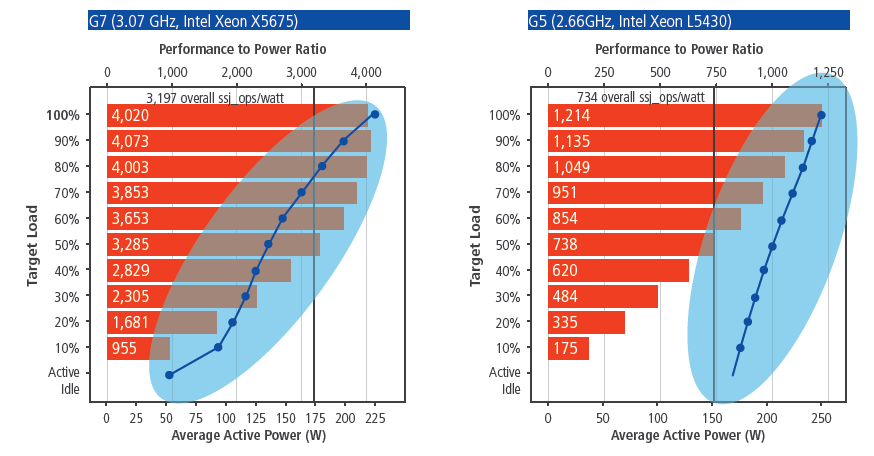
\includegraphics[width=0.8\textwidth]{figures/server_power_consumption.PNG}
	\caption{Server power consumption}
	\label{fig:server_power_consumption}
\end{figure}


\end{itemize}


\section{Forecasting}

\subsection{Definition}

A very general definition of forecasting and its prerequisites is given here\footnote{O-Texts \url{https://www.otexts.org/fpp/1/1}}:

\begin{quote}
The predictability of an event or a quantity depends on several factors including:

\begin{itemize}
\item how well we understand the factors that contribute to it
\item how much data are available
\item whether the forecasts can affect the thing we are trying to forecast
\end{itemize}
\end{quote}


\subsection{Types of forecasting}

%Forecasting can be done in different ways, each having their own drawbacks and benefits. 

Forecasting methods can be classified into two categories: Qualitative and Quantitative forecasting. 

\subsubsection{Qualitative forecasting}
Qualitative forecasting methods assume that there is no or no relevant data that can be used to make forecasts. This is the case for forecasts that aim to predict i.e. the first year's sales of a new product line or the expected profit of a newly created startup company. In both examples there is no data available beforehand and the forecast has to be derived from already known conditions also called predictor variables. 

\subsubsection{Quantitative forecasting}
Qantitative forecasting methods are based on numerical historical data, from which forecasts are derived. It is assumed that the data�s pattern over time stays the same or will behave in a similar way in the future. 

Quantitative forecasting methods can again be classified roughly into two categories: Cross-sectional forecasting and Time Series forecasting. 

\begin{itemize}
\item Cross-sectional forecasts collect data from a single point in time to predict a value for an item not in the dataset. For example, prices of real estates in a specific area and point in time are collected and the price for another real estate is estimated based on predictor variables (i.e., size of properties and number of floors). 

\item Time series forecasts are solely based on historical data from the value to be predicted. No other variables are considered for the calculation, which on the one hand might miss some influential factors from external conditions but on the other hand appears to be more accurate regarding the output of the forecasts. 
In case of energy price forecasts external variables that change energy price behavior might include bids in auctions of wholesale energy markets, the current oil price or availability of renewable energy sources. However, in time series forecasts these variables are neglected to set the focus on the time series of historical energy prices. 
\end{itemize}


\subsection{Forecast accuracy}

There are different kinds of accuracy measures that can be applied to forecasting methods. \footnote{https://www.otexts.org/fpp/2/5}

\subsubsection{Scale-dependent error measures}

Scale dependent errors are absolute error measures given in the same scale as the dataset that is examined. Thus they are most useful when testing fc methods on the same dataset or on the same scale, respectively. 

\begin{itemize}
\item Mean absolute error (MAE)
The absolute error is defined by the value difference between a value of the dataset and its forecasted value. The mean absolute error returns the mean of all absolute errors on the dataset. [insert formula]

\item Root mean squared error (RMSE)
The root mean squared error takes the root of the sum of the squared forecast errors, and is scale dependent as well. [insert formula]

\end{itemize}

\subsubsection{Percentage error measures}

The most common percentage error is the mean absolute percentage error (MAPE) which is defined as the mean of percentage errors of a dataset. A percentage error is defined as $p_i=e_i/y_i * 100$. The mean absolute percentage error is then $mean(|pi|)$. 

The disadvantage of percentage error measures is that the value becomes infinite if there is some $y_i = 0$ on the dataset. Also, extreme values occur when the values on the dataset come close to zero. 



\subsection{Forecast models}

\subsubsection{ARIMA models}


\subsubsection{Exponential Smoothing models}


\subsection{Forecast model evaluation}

\subsubsection{Tests for appropriateness of forecasting models}

If a model has been chosen, it needs to be tested to ensure its applicability for the given dataset. 



\section{Time Series Processing}

\subsection{Decomposition of time series}

Decomposition of time series can be helpful to determine various trends and patterns in the dataset. Based on recognized patterns and a thorough analysis of the data�s behavior and characteristics an appropriate forecasting model can be chosen. 

A time series exhibiting a trend, seasonal variations and random fluctuations can be decomposed into a trend component, seasonal component and irregular component, respectively. 







\section{Simulation}

\subsection{Data Center Locations}

Data center locations have been chosen such that they are placed in areas where a wholesale electricity market is available. For some locations data has been generated based on distribution of data in actual power markets. 

Price and temperature data is available for the following locations throughout the year 2010: 

Belgium - St. Ghislain

Singapore - Singapore

Taiwan - Changhua County

Indiana - Indianapolis

Michigan - Detroit

\subsection{Power markets}

Various power markets exist that provide data about historical energy prices. For simplicity, real data was taken for locations in the US and based on that generated for the other locations. The prices have been normalized to values between 0 and 1 based on maximum and minimum values in the dataset. Therefore, prices can be compared directly and do not need to be converted. 

\subsection{Parameters}

\begin{itemize}
\item Migration Overhead / Costs

\item On/Off Peak Prices

\item different Time Zones
		
\item Cooling depending on outside temperatures
		
\item Types of workload - short / long running jobs
		
\item Elasticity level of servers
		
\item Type(s) of forecasting - short term, mid term, long term

\item Minimum number of VMs to migrate in order to amortize migration costs

\item Possible consideration of different energy sources - renewables, atom, fossils

\end{itemize}


\subsection{Dynamic request routing}

\begin{itemize}

\item Load balancing of data of requests over all data centers

\item Determination of the currently cheapest data center

\item Possibly combined with forecasting energy prices

\item Integrating load forecasting as an additional measure

\item Estimation of DC load based on current DC load

\end{itemize}

\subsection{VM Migration}

\begin{itemize}

\item Minimum job duration for amortization of costs

\item Same VM / DC Selection Mechanism as with dynamic request routing

\end{itemize}

\subsection{Simulation models}

\begin{itemize}

\item Create scenarios both with and without forecasting

\item Evaluation of simulation results, overall power consumption/costs

\item Mapping power consumption to energy costs

\item Derive power consumption based on CPU load and possibly other parameters. Depends on elasticity

\item Model migration costs, depending on the workload

\end{itemize}



\section{Methodology}


\subsection{Forecasting}

\subsubsection{Forecast error classification}

\begin{itemize}

\item Mean absolute error (MAE): \[ \frac{1}{n} \sum_{i=1}^{n} |\hat{y}_i - y_i| \] % \[\sum_{i=1}^{10} t_i\] %\sum(abs(predicted - actual)) / N

\item Mean squared error (MSE): \[ \frac{1}{n} \sum_{i=1}^{n} (\hat{y}_i - y_i)^2 \] %$sum((predicted - actual)^2) / N$

\item Root mean squared error (RMSE): \[ \sqrt{\frac{1}{n} \sum_{i=1}^{n} (\hat{y}_i - y_i)^2}\] % $sqrt(sum((predicted - actual)^2) / N)$

\item Mean absolute percentage error (MAPE): \[ \frac{1}{n} \sum_{i=1}^{n} \left|\frac{\hat{y}_i - y_i}{y_i}\right| \] % $sum(abs((predicted - actual) / actual)) / N$

\item Direction accuracy (DAC): \[ \frac{count(sign(y_i - y_{i-1}) = sign(\hat{y}_i - \hat{y}_{i-1}))}{n} \]
% $count(sign(actual\_current - actual\_previous) == sign(pred\_current - pred\_previous)) / N$

\item Relative absolute error (RAE): \[  \frac{ \sum_{i=1}^{n} |\hat{y}_i - y_i|}{ \sum_{i=1}^{n} |\hat{y}_{i-1} - y_i|}   \]
 % $sum(abs(predicted - actual)) / sum(abs(previous\_target - actual))$

\item Root relative squared error (RRSE): \[  \frac{ \sqrt{ \frac{1}{n} \sum_{i=1}^{n} (\hat{y}_i - y_i)^2 }} { \sqrt{ \frac{1}{n} \sum_{i=1}^{n} (\hat{y}_{i-1} - y_i)^2 }} \]
 % $sqrt(sum((predicted - actual)^2) / N) / sqrt(sum(previous\_target - actual)^2 / N)$

\end{itemize}


\subsubsection{White noise tests for residuals}

To test if residuals can be regarded as white noise, its auto correlation functions is examined. In case auto correlations are present it means that some values within the series depend on one another. In theory a true white noise series should not exhibit any auto correlations but since we operate on finite time series there will always be a few correlations present in the data\cite{makridakisforecasting}. 

It can be shown that the auto correlations of a white noise series have a sampling distribution similar to a gaussian distribution with zero mean and a standard deviation of $1/\sqrt{n}$ where $n$ denotes the total number of observations in the series\cite{makridakisforecasting}. 

\subsection{General forecasting procedure}

\begin{itemize}

\item Selection of data sets (location, frequency)

\item Investigation of characteristics of the selected data sets (stationarity, variance)

\item Making series stationary on demand

\item Evaluation of appropriate models to be applied to the given data sets

\item Model generation based on evaluation

\item Model evaluation and comparison (goodness of fit, accuracy, residual characteristics) 

\item Tests on in-sample and out-of-sample data

\item Testing different forecasting horizons

\item Comparison of results for different time sets and locations

\item Conclusion and model selection based on results

\end{itemize}

\subsection{Forecasting workflow}




\subsection{Dynamic model selection}

Different energy markets show different characteristics in their time series of energy price data, i.e.\ seasonal or non-seasonal behavior or strong or weak probability of energy spike occurrence within a given time frame. Depending on these characteristics different forecasting models may be chosen s.t. they accommodate the behavior of the time series. 
However there are still minor changes in characteristics of time series within the same energy market so that it is generally not possible to identify a single model that is optimized for all energy price time series of a market. 
Depending on the given time frame and the selected series a different model may be selected. The criteria for model selection are its residual behavior (white noise characteristics) and parameter estimation as described in section []. 

When energy price data is provided to the simulator (and further to the forecasting plugin) it is first checked on its characteristics to determine a suitable model for this kind of data. Different types of models can be predetermined among which the best model will be chosen based on its residual and forecasting behavior. 



\printbibliography


\end{document}